% Brian Mc George - MCGBRI004
% Jacques Heunis - HNSJAC003
% Timothy Gwynn - GWNTIM001
% Due: 31-07-2015
% Stage One - Software Engineering  - CSC3003S
\documentclass[a4paper,10pt]{article}
%**************************************************************************************************
% PACKAGES
%**************************************************************************************************
\usepackage{amsmath, amsthm, amsfonts, amssymb}
\usepackage{graphicx,color}
\usepackage{bm}	
\usepackage{float}
\usepackage{caption, subcaption}
%\usepackage{vector}

%**************************************************************************************************
% DEFAULT SETTINGS
%**************************************************************************************************
\marginparwidth -20 true pt    % Width of marginal notes.
\oddsidemargin  -10 true pt       % Note that \oddsidemargin=\evensidemargin
\evensidemargin -10 true pt
\topmargin -0.5 true in        % Nominal distance from top of page to top of
\textheight 9.75 true in         % Height of text (including footnotes and figures)
\textwidth 7 true in        % Width of text line.
\parindent=10pt                  % Do not indent paragraphs
\parskip= 1 ex
\columnseprule = 0.1pt
\footskip = 30 true pt
\hoffset = -0.1 true in
\voffset = -0.1 true in
\abovedisplayskip 1 true pt
\abovedisplayshortskip 1 true pt
\topsep 0 true pt
\newcommand*\varhrulefill[1][0.4pt]{\leavevmode\leaders\hrule height#1\hfill\kern0pt}

%**************************************************************************************************
% DOCUMENT DETAILS
%**************************************************************************************************


%**************************************************************************************************
% MAIN DOCUMENT 
%**************************************************************************************************

\begin{document}
\begin{titlepage} \begin{center} 
		\textsc{\LARGE University of Cape Town}
		\\[1.5cm] \textsc{\Large Software Engineering Stage One\\CSC3003S}
		\\[0.5cm]
		\noindent\rule[0.4mm]{\textwidth}{0.1mm}
		\\[0.4cm] { \huge \bfseries Tempest Trace \\[0.4cm] }
		\noindent\rule[0.4mm]{\textwidth}{0.1mm}
		\\[1cm]
		\begin{minipage}[t]{0.4\textwidth}
		\begin{flushleft}\large \emph{Authors:}\\ Brian Mc George - MCGBRI004 \\ Jacques Heunis - HNSJAC003 \\ Timothy Gwynn - GWYTIM001\end{flushleft}
		 \end{minipage} \begin{minipage}[t]{0.4\textwidth} 
		\begin{flushright} \large \emph{Supervisor:} \\ Assoc. Prof.~Patrick Marais\\patrick@cs.uct.ac.za\end{flushright}
		\begin{flushright} \large \emph{Tutor:} \\ Codie Roelf\\Codie.Roelf@alumni.uct.ac.za\end{flushright}
		 \end{minipage} \vfill {\large \today}
		\end{center}
		\end{titlepage}
\newpage
\tableofcontents
\newpage

\section{Use Case Narratives}
\subsection{Player Movement}
Actor: Player\\\\
The player specifies which direction he/she wants the character to move in. The system performs collision detection to detect whether the input movement is allowed. If the movement is allowed the player's character is appropriately displaced in the system and the appropriate animation is played. The system represents this graphically for both players. The system makes updates the AI behaviour based on the new position of the player. The system checks whether the player has reached the end goal and if so ends the game.\\\\
If the movement is not allowed the player's character will not move and no adjustments will be made to the system.
\subsection{Player Jump}
Actor: Player\\\\
The player specifies he/she wants the character to jump. The system performs collision detection to detect whether the input movement is allowed. If the movement is allowed the player's character is appropriately displaced in the system depending on what sort of obstacle is in close proximity and in front of the player and the appropriate animation is played. The system represents this graphically for both players. The system makes updates the AI behaviour based on the new position of the player. The system checks whether the player has reached the end goal and if so ends the game.\\\\
If the movement is not allowed the player's character will not move and no adjustments will be made to the system.
\subsection{Player Slide}
Actor: Player\\\\
The player specifies he/she wants the character to slide. The system performs collision detection to detect whether the input movement is allowed. If the movement is allowed the player's character is appropriately displaced in the system depending on what slope is in front of the player and the appropriate animation is played. The system represents this graphically for both players. The system makes updates the AI behaviour based on the new position of the player. The system checks whether the player has reached the end goal and if so ends the game.\\\\
If the movement is not allowed the player's character will not move and no adjustments will be made to the system.
\subsection{Player Respawn}
Actor: Player\\\\
The player's character dies. The system checks where the closest respawn point behind the player is. If there are no obstacles at the spawn location the player's character appears at the location and the appropriate animation is played. The system represents this graphically for both players and updates the player's character's location.  The system makes updates the AI behaviour based on the new position of the player. \\\\
If the spawn location is blocked, prehaps by the other player or an AI unit the game will delay the respawn up to 1.5 seconds until the spawn location is cleared otherwise it will pick the next closest spawn location.
\newpage
\subsection{AI Behaviour}
Actor: Time\\\\
Every 5 seconds the AI updates it's behaviour. The AI checks with the system whether it has a target, if it has a target it then checks whether that target is in line of sight, if the target is in line of sight then the ai moves towards the target and shoots towards it if it is in range. If the target is not in line of sight the AI checks whether the other possible target is in line of sight, if this is the case it will switch targets, otherwise it will proceed to it's cureent target's last seen position. If the AI has no target it will continue to patrol between predifined points until a tartget enters line of sight at which point the system will assign the AI the target.

\section{Analysis Class Model}
\begin{figure}[H]
	\begin{center}
		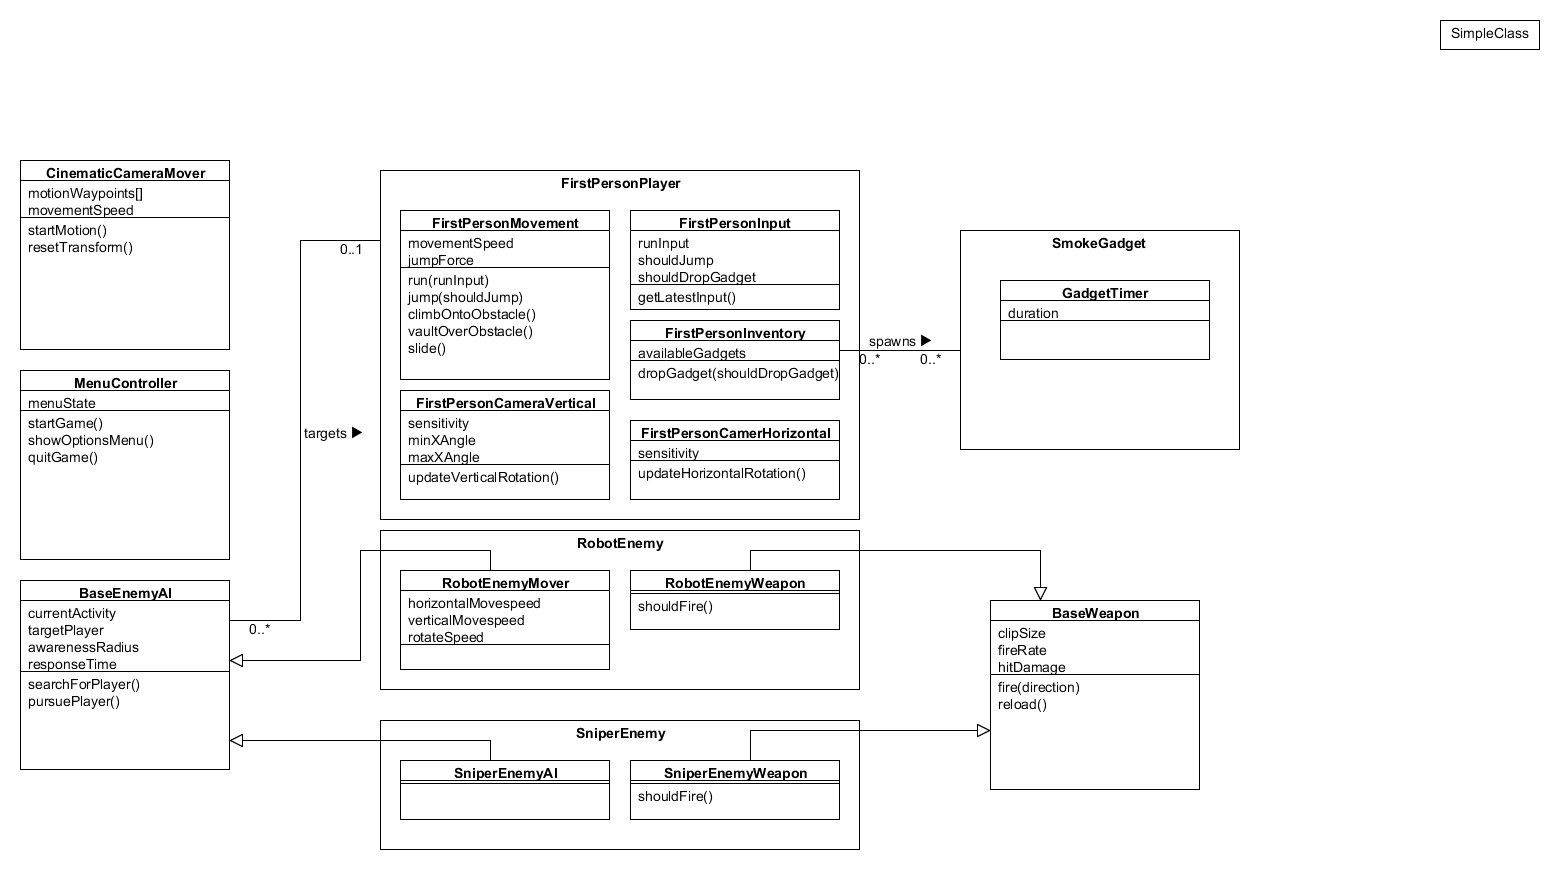
\includegraphics[scale=0.4]{images/AnalysisClassDiagram.png}
		\caption{Get analysisized!}
	\end{center}
\end{figure}
A first-draft analysis class model.

\section{State Diagrams}
\begin{figure}[H]
	\begin{center}
		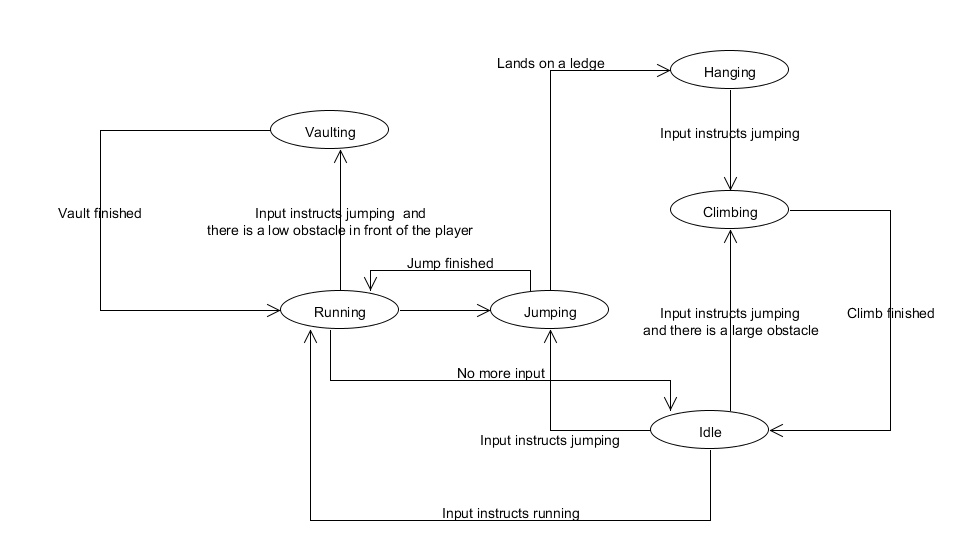
\includegraphics[scale=0.4]{images/PlayerStateMachine.png}
		\caption{A state machine for the player}
	\end{center}
\end{figure}
\begin{figure}[H]
	\begin{center}
		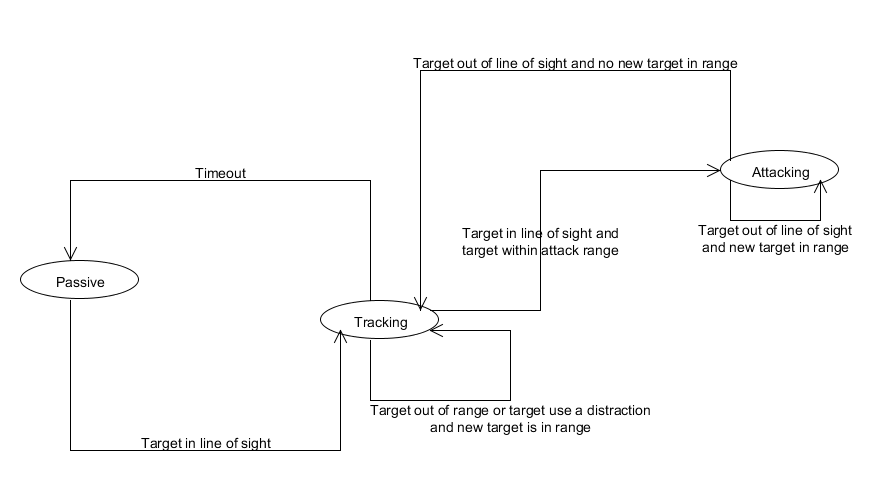
\includegraphics[scale=0.4]{images/EnemyStateMachine.png}
		\caption{A state machine for the 2 types of enemies in the game}
	\end{center}
\end{figure}

\section{Project Plan}

\section{Test Plan}

\end{document}
